\documentclass[aspectratio=169]{beamer}
\usepackage{graphicx}
\usepackage{amsmath}
\usepackage{amsthm}
\usepackage{amssymb}
\usepackage[T1]{fontenc}
\usepackage[utf8]{inputenc}
\usepackage[english]{babel}
\usepackage{bm}
\usepackage{hyperref}
\usepackage{xcolor}
\usepackage{booktabs}
\usepackage{soul}
\usepackage{algorithm2e}

\newcommand{\bruno}[1]{\textcolor{blue}{#1}} % Bruno Sanso edits- blue
\newcommand{\findcite}{{\color{red} [Find Citation]}}
\newcommand{\needcite}{\findcite}
\newcommand{\makenote}[1]{{\color{red} #1}}
\newcommand{\Chi}{\mbox{\Large$\chi$}}
\newcommand{\norm}[1]{\left\lVert #1 \right\rVert}
\newcommand{\inorm}[1]{\norm{#1}_{\infty}}
\newcommand{\pnorm}[2]{\norm{#1}_{#2}}

\newtheorem{prop}{Proposition}

\DeclareMathOperator{\tr}{Tr}
\DeclareMathOperator*{\argmin}{arg\,min}
\DeclareMathOperator*{\argmax}{arg\,max}



\title{Multivariate Extreme Value Theory and Applications to Anomaly Detection}
\author{Peter Trubey \\ UCSC Department of Statistics}
\date[8/25/2021]{Advancement}

\begin{document}

\begin{frame}
  \titlepage
\end{frame}

\begin{frame}
  \frametitle{Overview}
  \tableofcontents
\end{frame}

\section{Introduction}

\begin{frame}
  \frametitle{Introduction}


\end{frame}



\subsection{Extreme Value Theory}

\begin{frame}
  \frametitle{EVT - A Brief Background}
  \begin{itemize}
    \item Why EVT?
    \item Block Maxima - GEV
    \item Thresholding - GP
  \end{itemize}
\end{frame}

\begin{frame}
  \frametitle{Block Maxima}
  For $x_i \stackrel{\text{iid}}{\sim} F$, Let $M_n = \max_{i} x_i$.
  \begin{equation*}
    \begin{aligned}
      \text{Pr}\left[M_n\leq z\right] &= \text{Pr}\left[X_1 \leq z, \ldots, X_n \leq z\right]\\
        &= \text{Pr}\left[X_1\leq z\right]\times\ldots\times\text{Pr}\left[X_n\leq z\right]\\
        &= F(z)^n.
    \end{aligned}
  \end{equation*}
  But if $F$ is unknown?

  How to keep from degenerating to a point mass?
\end{frame}

\begin{frame}
  \frametitle{Block Maxima - Fisher-Tippett-Gnedenko Theorem}
  If there exists a sequence of constants $a_n > 0$, $b_n$ such that:
  \begin{equation*}
    \text{Pr}\left[\frac{M_n - b_n}{a_n} \leq z\right] \stackrel{d}{\rightarrow} G(z)
  \end{equation*}
  as $n\to\infty$,

  Then $G$ is a \emph{max-stable distribution}, and $F$ is in its \emph{domain of attraction}.
\end{frame}

\begin{frame}
  \frametitle{Block Maxima - GEV}
  \begin{itemize}
    \item 3 possible forms for these max stable distributions\\
      \hspace{1cm}Fr{\'e}chet, Gumbel, and Weibull
    \pause
    \item One unifying form
      \begin{equation*}
        F(m \mid \mu, \sigma, \xi) = \exp\left\lbrace-\left[1 +
              \xi\left(\frac{x - \mu}{\sigma}\right)\right]_{}^{-1/{\xi}}\right\rbrace.
      \end{equation*}
      the \emph{generalized extreme value distribution}
  \end{itemize}
\end{frame}

\begin{frame}
  \frametitle{Block Maxima - Inference}
  \begin{itemize}
    \item Inference requires blocking data and taking maximum within a block
    \pause
    \item Reduces data for inference to $1 / \text{block size}$.
    \pause
    \item Ignore those pesky \emph{iid} requirements
  \end{itemize}
\end{frame}

\begin{frame}
  \frametitle{Thresholding - Pickands-Balkema-de Haan Theorem}
  \begin{itemize}
    \item For $X \sim F$:
      \begin{equation*}
        \text{Pr}\left[X > u + y\mid X > u\right] = \frac{1 - F(u + y)}{1 - F(u)}.
      \end{equation*}
    \pause
    \item If $F$ is in the domain of the GEV:
      \begin{equation*}
        \lim\limits_{u\to u^{\prime}}\text{Pr}\left[X > u + y\mid X > u\right] = H(y)
      \end{equation*}
  \end{itemize}
\end{frame}

\begin{frame}
  \frametitle{Thresholding - Generalized Pareto}

\end{frame}


\begin{frame}
  \frametitle{Multivariate EVT}
  \begin{itemize}
    \item Useful to standardize each $X_i$ according to its marginal distribution
    \item Standardization occcurs as:
      \begin{equation}
        z_j = \left(1 + \xi\frac{x_j - b_{t,j}}{a_{t,j}}\right)_{+}^{1/\xi}
      \end{equation}
			where $b_{t,j} = \hat{F}^{-1}(1 - 1/t)$.
    \item Note that $Z_j > 1\implies X_j > b_{t,j}$
    \item $\max_j Z_j \sim \text{Pareto}$
		\item $a$, $\xi$ are currently found by MLE.  Not ideal, I know.
  \end{itemize}
\end{frame}

\begin{frame}
  \frametitle{Multivariate EVT}
  \begin{itemize}
    \item Assume the existence of a limit measure $\mu$ on ${\bf Z}$ such that:
    \begin{equation*}
      n\text{Pr}\left(\frac{V_1}{n} \geq v_1 \text{ or }\ldots\text{ or }\frac{V_d}{n}\geq v_d\right)
      \rightarrow \mu\left([{\bf 0}, {\bf v}]^C\right)
    \end{equation*}
    \item $\mu$ is the asymptotic distribution of ${\bf Z}$ in extreme regions.
    \item $\mu$ features the homogeneity property, $\mu(t\cdot) = t^{-1}\mu(\cdot)$.
  \end{itemize}
\end{frame}

\begin{frame}
  \frametitle{Spectral Measure}
  For $B \subset S_{\infty}^{d-1}$, define the \emph{Spectral Measure}:
  \begin{equation*}
    \Omega(B) = \mu[{\bf z}: R({\bf z}) > 1, {\bf V} \in B].
  \end{equation*}
  Then,
  \begin{equation*}
    \mu[{\bf z}:R(z)>t, {\bf V}\in B] = t^{-1}\Omega(B).
  \end{equation*}
  Thus $t$ is independent of $\Omega$, the spectral measure.  This is completed as a
    probability measure as:
  \begin{equation*}
    \text{Pr}\left({\bf V} \in B \mid r > 1\right) = \frac{\Omega(B)}{\Omega(S_{\infty}^{d-1})}.
  \end{equation*}
  So conditional on at least one dimension exceeding its threshold, we can hold the
  angular measure independent of the magnitude.
\end{frame}

\subsection{Integrated Vapor Transport}
\begin{frame}
  \frametitle{Integrated Vapor Transport}
\end{frame}

\section{Methodology}

\begin{frame}
  \frametitle{Casting \emph{real} data to $\mathcal{S}_{\infty}^{d-1}$}
\end{frame}

\subsection{Projection onto $\mathcal{S}_{\infty}^{d-1}$}

\begin{frame}
  \frametitle{The Unit Sphere}
  \begin{columns}
    \begin{column}{.48\textwidth}
      \begin{itemize}
        \item $\mathcal{L}_p$ Norm:
          \begin{equation*}
            \lVert \bm{s}\rVert_p = \left[\sum_{l = 1}^ds_l^p\right]^{\frac{1}{p}}
          \end{equation*}
        \pause
        \item Unit Sphere on $\mathcal{L}_p$ Norm
          \begin{equation*}
            \mathcal{S}_{p}^{d-1} = \left\lbrace \bm{s} : \lVert\bm{s}\rVert_p = 1 \right\rbrace
          \end{equation*}
      \end{itemize}
    \end{column}%
    \hfill%
    \pause
    \begin{column}{.48\textwidth}
      \begin{center}
        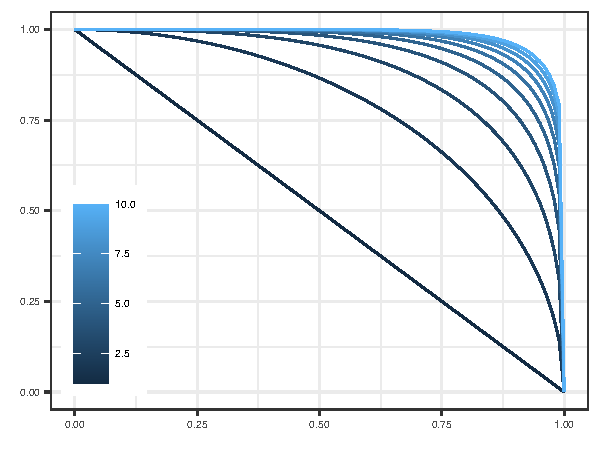
\includegraphics{./images/p_sphere}
      \end{center}
    \end{column}%
  \end{columns}%
\end{frame}

\begin{frame}
  \frametitle{Projection onto the Unit Norm Sphere}
  \begin{itemize}
    \item Take a distribution from $\mathcal{R}_+^{d}$ to $\mathcal{S}_{p}^{d-1}$
    \pause
    \item For finite $p$
      \begin{equation*}
        y_d = \left(1 - {\textstyle\sum}_{l = 1}^{d-1}y_l^p\right)^{\frac{1}{p}}
      \end{equation*}
    \pause
    \item Transformation to Radial, Angular
    \begin{equation*}
      T(x_1,\ldots,x_d) = \left(\pnorm{\bm{x}}{p}, \frac{x_1}{\pnorm{\bm{x}}{p}},
                    \ldots , \frac{x_{d-1}}{\pnorm{\bm{x}}{p}}\right) = (r,y_1,\ldots,y_{d-1})
    \end{equation*}
    \pause
    \begin{equation*}
    T^{-1}\left(r,y_1,\ldots,y_{d-1}\right) =
      \left(ry_1,\ldots,ry_{d-1}, r\left(1 - {\textstyle\sum}_{l = 1}^{d-1}y_l^p\right)^{\frac{1}{p}}\right)
    \end{equation*}
  \end{itemize}
\end{frame}

\begin{frame}
  \frametitle{Projection - Jacobian}
  \begin{equation*}
    \begin{bmatrix}
      y_1 & r & 0 & \ldots & 0\\
      y_2 & 0 & r & \ldots & 0\\
      \vdots & \vdots & \vdots & \ddots & \vdots\\
      y_{d-1} & 0 & \ldots & 0 & r \\
      \left(1 - {\scriptsize\sum_{l=1}^{d-1}}y_l^p\right)^{1/p} &
        - y_1^{p-1}\phi & -y_2^{p-1}\phi & \cdots & -y_{d-1}\phi
    \end{bmatrix}
  \end{equation*}
  where $\phi = \left(1 - {\scriptsize\sum_{l=1}^{d-1}}y_l^p\right)^{1/p - 1}$
  \pause
  \begin{equation*}
  \lvert J \rvert = r^{d-1}\left[\left(1 - {\textstyle\sum}_{l = 1}^{d-1}y_l^p\right)^{\frac{1}{p}} +
      {\textstyle\sum}_{l = 1}^{d-1}y_l^p\left(1 - {\textstyle\sum}_{l=1}^{d-1}
          y_l^p\right)^{\frac{1}{p} - 1}\right].
  \end{equation*}
\end{frame}

\subsection{Projected Gamma Family}

\begin{frame}
  \frametitle{Projected Gamma Distribution}
  \begin{itemize}
    \item Assume a product of independent Gammas
      \begin{equation*}
        f(r,\bm{y}) = \prod_{l = 1}^d \text{Ga}\left(ry_l\mid\alpha_l,\beta_l\right)
        \lvert J \rvert I_{\bm{y} \in \mathcal{S}_{p}^{d-1}}
      \end{equation*}
    \pause
    \item Expanded Form
      \begin{equation*}
        f(r,\bm{ y}) = \prod_{l = 1}^{d}
        \left[\frac{\beta_l^{\alpha_l}}{\Gamma(\alpha_l)}(ry_l)^{\alpha_l - 1}
                    \exp\lbrace-\beta_lry_l\rbrace\right]
        \times r^{d-1}\left[y_d - {\textstyle \sum}_{l = 1}^{d-1}y_l^p
                  \left(y_d^p\right)^{\frac{1}{p} - 1}\right]
      \end{equation*}
    \pause
    \item Integrate out radial component; left with distribution on angular
      \begin{equation*}
        \text{PG}(\bm{ y}\mid\bm{ \alpha},\bm{ \beta}) = \prod_{l = 1}^d\left[\frac{\beta_l^{\alpha_l}}{\Gamma(\alpha_l)}y_l^{\alpha_l - 1}\right]
          \times \left[y_d - {\textstyle \sum}_{l = 1}^{d-1}y_l^p\left(y_d^p\right)^{\frac{1}{p} - 1}\right]
          \times \frac{\Gamma({\textstyle\sum}_{l = 1}^d\alpha_l)}{\left({\textstyle\sum}_{l = 1}^d \beta_ly_l\right)^{{\scriptstyle\sum_{l = 1}^d \alpha_l}}}
      \end{equation*}
  \end{itemize}
\end{frame}

\begin{frame}
  \frametitle{Data augmentation}
  \begin{itemize}
    \item Sample from full conditional for $r$
      \begin{equation*}
        r\mid\bm{ \alpha},\bm{ \beta}, y \sim \text{Ga}\left(r\mid{\textstyle\sum}_{l = 1}^d \alpha_l,
              {\textstyle\sum}_{l = 1}^d \beta_ly_l\right).
      \end{equation*}
    \pause
    \item To recover independent Gammas interetation
      \begin{equation*}
        L(\bm{\alpha},\bm{\beta} \mid \bm{r},\bm{y}) \propto
            \prod_{i = 1}^n\prod_{l = 1}^{d}\text{Ga}\left(r_iy_{il}\mid\alpha_l,\beta_l\right)
      \end{equation*}
    \pause
    \item Enabling independent inference between columns
      \begin{equation*}
        L(\alpha_l,\beta_l) \propto \prod_{i = 1}^n
                  \text{Ga}\left(r_iy_{il}\mid\alpha_l,\beta_l\right)
      \end{equation*}
  \end{itemize}
\end{frame}

\begin{frame}
  \frametitle{Projected Gamma Model}
  \begin{equation*}
    \begin{aligned}
      \bm{ y}\mid\alpha,\beta &\sim \text{PG}(\bm{ y}\mid\alpha,\beta)\\
      \bm{ \alpha},\bm{\beta} &\sim {\textstyle \prod}_{l = 1}^d \text{Ga}(\alpha_l \mid \xi_l,\tau_l)
              \times {\textstyle \prod}_{l = 2}^d \text{Ga}(\beta_l\mid \zeta_l,\sigma_l).
    \end{aligned}
  \end{equation*}
\end{frame}

\begin{frame}
  \frametitle{Projected Gamma Model - Inference}
  \begin{itemize}
    \item Full conditional for $\beta_l$
      \begin{equation*}
        \beta_l\mid \bm{ y}, r, \alpha_l \sim \text{Ga}\left(n + \alpha_l + \zeta_l,
                {\textstyle \sum}_{i = 1}^nr_iy_{il} + \sigma_l\right)
      \end{equation*}
    \pause
    \item Log-posterior for $\alpha_l$
      \begin{equation*}
        f(\alpha_l \mid \bm{ y}, r) \propto
          \frac{\left({\textstyle \prod}_{i = 1}^nr_iy_{il}\right)^{\alpha_l - 1}}{
            \Gamma^n(\alpha_l)} \times \alpha_l^{\xi_l - 1}\exp\{-\tau_l\alpha_l\} \times
            \frac{\Gamma(n\alpha_l + \zeta_l)}{
            \left({\textstyle\sum}_{i = 1}^n r_iy_{il} + \sigma_l
                  \right)^{(n * \alpha_l + \zeta_l)}}
      \end{equation*}
    \pause
    \item If $\beta_l = 1$, then
    \begin{equation*}
      f(\alpha_1 \mid \bm{ y}, r) \propto
        \frac{{\textstyle\prod}_{i = 1}^n ry_{i1}^{\alpha_1 - 1}}{\Gamma^n(\alpha_1)} \times
        \alpha_1^{\xi_1 - 1}\exp\{-\tau_1\alpha_1\}
    \end{equation*}
  \end{itemize}
\end{frame}

\begin{frame}
  \frametitle{Finite Mixture Model}
  \begin{equation*}
    \begin{aligned}
      \bm{ y}_i &\sim \sum_{j = 1}^J\pi_j\text{PG}\left(\bm{ y}\mid \bm{ \alpha}_j, \bm{ \beta}_j\right)\\
      \bm{ \alpha}_j &\sim {\textstyle \prod}_{l = 1}^d \text{Ga}\left(\alpha_l\mid\xi_l,\tau_l\right)\\
      \bm{ \beta}_j &\sim {\textstyle \prod}_{l = 2}^d \text{Ga}\left(\beta_l\mid\zeta_l,\sigma_l\right)
    \end{aligned}
    \hspace{2cm}
    \begin{aligned}
      \bm{ \xi},\bm{\tau} &\sim {\textstyle \prod}_{l = 1}^d \text{Ga}(\xi_l\mid a,b)
                \times \text{Ga}(\tau_l\mid c,d)\\
      \bm{ \zeta},\bm{\sigma} &\sim {\textstyle\prod}_{l = 2}^d\text{Ga}(\zeta_l \mid a,b)
              \times \text{Ga}(\sigma_l\mid c,d)\\
      \bm{ \pi} &\sim \text{Dir}(\pi_0)
    \end{aligned}
  \end{equation*}
\end{frame}

\begin{frame}
  \frametitle{Dirichlet Process Mixture Model}
  \begin{equation*}
    \begin{aligned}
      \bm{ y}_i &\sim \sum_{j = 1}^J\pi_j\text{PG}\left(\bm{ y}\mid \bm{ \alpha}_i, \bm{ \beta}_i\right)\\
      (\alpha_i,\beta_i) &\sim \text{DP}\left(\eta, G_0\right)\\
      &~\hspace{-2cm}G_0 = {\textstyle\prod}_{l = 1}^d\text{Ga}\left(\alpha_{jl}\mid\xi_{l},\tau_{l}\right)
                    \times{\textstyle\prod}_{l=2}^d\text{Ga}\left(\beta_{jl}\mid\zeta_{l}\tau_{l}\right)
    \end{aligned}
    \hspace{1cm}
    \begin{aligned}
      \bm{ \xi},\bm{ \tau} &\sim {\textstyle \prod}_{l = 1}^d \text{Ga}(\xi_l\mid a,b)
              \times \text{Ga}(\tau_l\mid c,d)\\
      \bm{ \zeta},\bm{\sigma} &\sim {\textstyle\prod}_{l = 2}^d\text{Ga}(\zeta_l \mid a,b)
              \times \text{Ga}(\sigma_l\mid c,d)\\
      \bm{ \eta} &\sim \text{Ga}(\eta \mid 2, 0.1).
    \end{aligned}
  \end{equation*}
\end{frame}

\begin{frame}
  \frametitle{Log-normal Prior for Shape Parameters}
  \begin{equation*}
    \begin{aligned}
      \bm{ y}_i &\sim \sum_{j = 1}^J\pi_j\text{PG}\left(\bm{ y}\mid \bm{ \alpha}_i, \bm{\beta}_i\right)\\
      (\bm{\alpha}_i, \bm{\beta}_i) &\sim \text{DP}\left(\eta, G_0\right)\\
        &~\hspace{-1cm}G_0 = \mathcal{N}\left(\log\bm{ \alpha}_{j}\mid\mu,\Sigma\right)\times
            {\textstyle\prod}_{l = 2}^d\text{Ga}\left(\beta_{jl}\mid\zeta_l,\sigma_l\right)
    \end{aligned}
    \hspace{1cm}
    \begin{aligned}
      \mu,\Sigma &\sim \mathcal{N}\left(\mu\mid\mu_0,\Sigma_0\right)
                                  \times \text{IG}\left(\nu,\Psi\right)\\
      \bm{ \zeta},\bm{\sigma} &\sim {\textstyle\prod}_{l = 2}^d\text{Ga}(\zeta_l \mid a,b)
                                \times \text{Ga}(\sigma_l \mid c,d) \\
      \bm{ \eta} &\sim \text{Ga}(\eta \mid 2, 0.1).
    \end{aligned}
  \end{equation*}
\end{frame}

\begin{frame}
  \frametitle{Choice of Norm}
  \begin{itemize}
    \item $\bm{V} \in \mathcal{S}_{\infty}^{d-1}$
    \pause
    \item Difficult to project distribution in $\mathcal{R}_+^{d}$ to $\mathcal{S}_{\infty}^{d-1}$
    \pause
    \item Easy to project distribution in $\mathcal{R}_+^{d}$ to $\mathcal{S}_{p}^{d-1}$ for any finite $p$
    \pause
    \item Project to $\mathcal{S}_{p}^{d-1}$ for large $p$, then project posterior predictive samples
  \end{itemize}
\end{frame}

\subsection{Alternative Geometries}

\begin{frame}
  \frametitle{Alternative Geometries}
  \begin{itemize}
    \item Coordinate system to describe $\mathcal{S}_p^{d-1}$ in $\omega^{d-1}$
    \item $\mathcal{L}_1$: Log-ratios
    \item $\mathcal{L}_2$: Spherical Coordinates
      \begin{equation}
        \label{eqn:spherical}
        \begin{aligned}
          y_1 &= \cos\theta_1\\
          y_l &= \left[{\textstyle\prod}_{k = 1}^{l-1}\sin\theta_k\right]\cos\theta_l
                                    \hspace{1cm}\text{for } l = 2,\ldots,d-1\\
          y_d &= {\textstyle\prod}_{k = 1}^{d-1}\sin\theta_k
        \end{aligned}
      \end{equation}
  \end{itemize}
\end{frame}

\begin{frame}
  \frametitle{Probit-Normal}
  Let $Q_i = \text{Probit}(2\theta_i / \pi)$, for $i = 1,\ldots,d-1$
  \begin{equation*}
    \begin{aligned}
                Q_i &\sim \mathcal{N}_{d-1}\left(\mu_i, \Sigma_i\right)\\
    \mu_i, \sigma_i &\sim \text{DP}(\eta, G_0)\\
                    &\hspace{-1cm}G_0 =
                      \mathcal{N}_{d-1}(\mu_i\mid\mu_0,\Sigma_0)\times \text{IW}(\Sigma_i\mid\nu,\Psi)
    \end{aligned}
    \hspace{1cm}
    \begin{aligned}
              \mu_0 &\sim \mathcal{N}_{d-1}\left({\bf u},{\bf S}\right)\\
           \Sigma_0 &\sim \text{IW}(\nu_0,\Psi_0)\\
               \eta &\sim \text{Ga}(\alpha, \beta)
    \end{aligned}
  \end{equation*}
\end{frame}

\section{Model Comparison on the hypercube}

\begin{frame}
  \frametitle{Model Comparison on the Hypercube}
  \begin{itemize}
    \item Posterior Predictive Loss
    \item Energy Score
    \item Kullbeck Liebler Divergence
  \end{itemize}
\end{frame}

\begin{frame}
  \frametitle{Energy Score}
  \begin{itemize}
    \item Generalization of CRPS to multiple dimensions
    \begin{equation}
      \label{eq:es}
      \text{ES}\left(P,x_i\right) =  \text{E}_p g\left(\bm{X}_i, \bm{x}_i\right)
                - \frac{1}{2}\text{E}_p g\left(\bm{X}_i,\bm{X}_i^{\prime}\right)
    \end{equation}
    \pause
    \item Where $g$ is a negative definite kernel\\
      Euclidean distance is most common
    \pause
    \item What is most appropriate on the hypercube?
  \end{itemize}
\end{frame}

% \begin{frame}
%   \frametitle{Distance on $\mathcal{S}_{\infty}^{d-1}$}
%   \begin{itemize}
%     \item Positive orthant of hypercube
%       \begin{equation*}
%         \mathcal{S}_{\infty}^{d-1} = \left\lbrace \bm{s}\hspace{0.1cm}:\hspace{0.1cm}s_i \in [0,1],
%                                                         \hspace{0.2cm} \max_i s_i = 1\right\rbrace
%       \end{equation*}
%     \pause
%     \item Distance on the hypercube
%   \end{itemize}
% \end{frame}

\begin{frame}
  \frametitle{Positive Orthant of $\mathcal{S}_{\infty}^{d-1}$}
  \begin{center}
    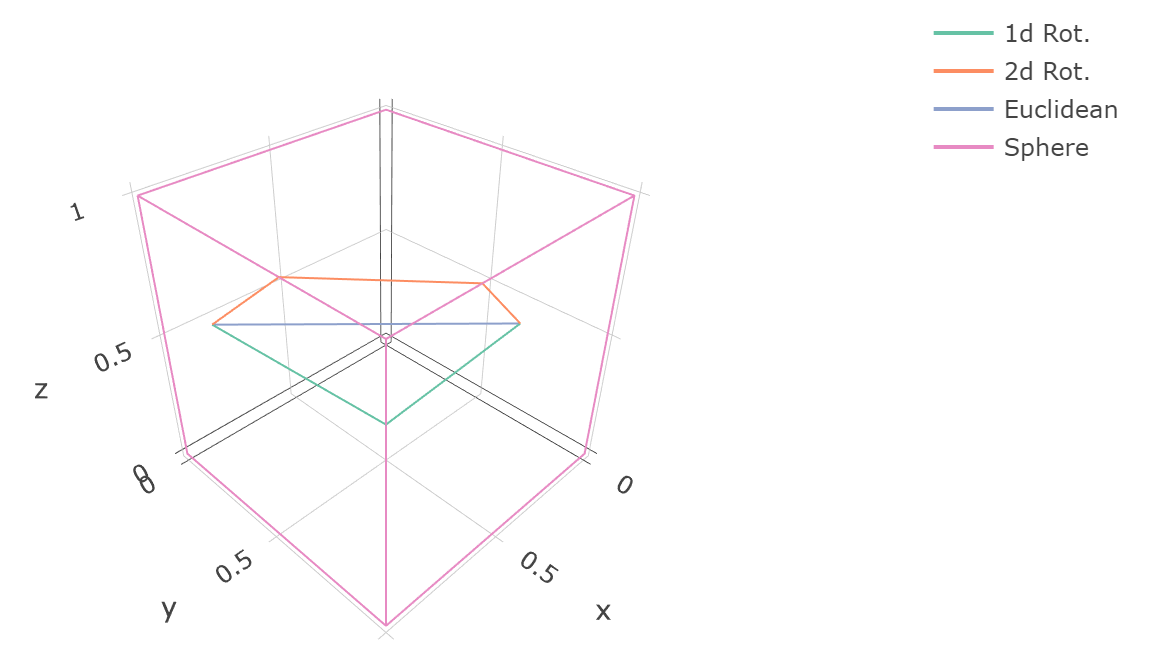
\includegraphics[width=0.9\linewidth]{./images/rotation}
  \end{center}
\end{frame}

\begin{frame}
  \frametitle{Distance on $\mathcal{S}_{\infty}^{d-1}$}
  \begin{itemize}
    \item Length of the shortest path between two points
    \pause
    \item A distance:
      \begin{itemize}
        \item is symmetric
        \item is positive
        \item respects triangle inequality
      \end{itemize}
  \end{itemize}
\end{frame}

\begin{frame}
  \frametitle{A Valid Negative Definite Kernel}
  \begin{prop}
    For points $a,b \in \mathcal{S}_{\infty}^{d-1}$ a valid negative definite kernel can be formed as
    \begin{equation*}
      g(\bm{a},\bm{b}) = \begin{cases}
        \pnorm{\bm{b}-\bm{a}}{2} &\text{ if }\argmax_l\bm{a} = \argmax_l\bm{b}\\
        \pnorm{\bm{c}-\bm{a}}{2} + \pnorm{\bm{b}-\bm{c}}{2} &\text{ otherwise}
      \end{cases}
    \end{equation*}
    where $\bm{c}$ resides on the intersection between the faces of $\bm{a}$ and $\bm{b}$, and
                minimizes $g(\bm{a},\bm{b})$.
  \end{prop}
\end{frame}

\begin{frame}
  \frametitle{Kullbeck Liebler Divergence}
  \begin{itemize}
    \item KL Divergence
      \begin{equation*}
        D_{\text{KL}}(A,B) = \int_{x\in \Omega(A)}A(x)\log\left(\frac{A(x)}{B(x)}\right)\text{d}x
      \end{equation*}
      requires an estimate of density
    \begin{item} D
    \begin{equation*}
        \label{eqn:knnkld}
        D_{\text{KL}}^{(k)}(A,B) = \log\frac{n(B)}{n(A)} + c(A) \left[\rho_A^{(k)}(B)
                                                          - \rho_A^{(k)}(A)\right]
    \end{equation*}
  \end{itemize}
\end{frame}


\section{Results}

\subsection{Simulation}

\begin{frame}
  \frametitle{Simulation Study}
  \begin{itemize}
    \item Finite mixture of Gammas
    \item For each Number of Mixture Components (3,6,9,12):
      \begin{itemize}
        \item Generate a data-set of 20 columns
        \item output subsets of c = 3,6,12,20 columns projected onto $\mathcal{S}_{\infty}^{c-1}$.
      \end{itemize}
  \end{itemize}
\end{frame}

\begin{frame}
  \frametitle{Simulation - Posterior predictive loss}
  \begin{center}
    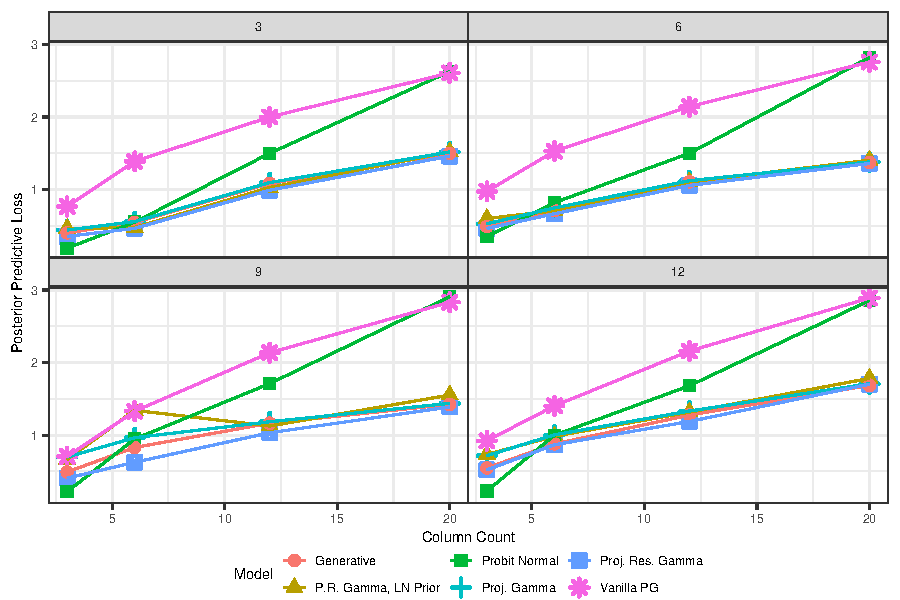
\includegraphics[width=0.9\linewidth]{./images/simulation_ppl}
  \end{center}
\end{frame}

\begin{frame}
  \frametitle{Simulation - Energy Score}
  \begin{center}
    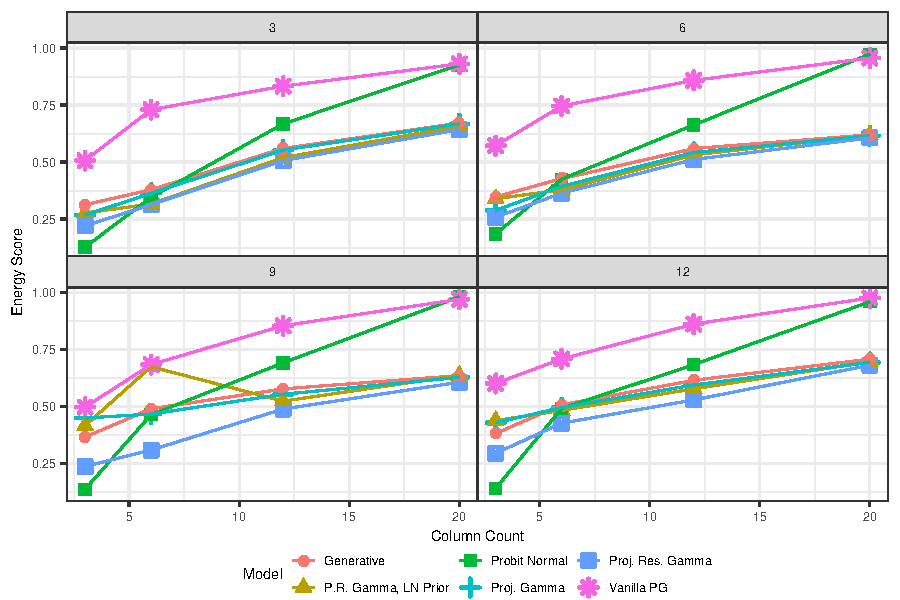
\includegraphics[width=0.9\linewidth]{./images/simulation_es}
  \end{center}
\end{Frame}

\begin{frame}
  \frametitle{Simulation - KL Divergence}
  \begin{center}
    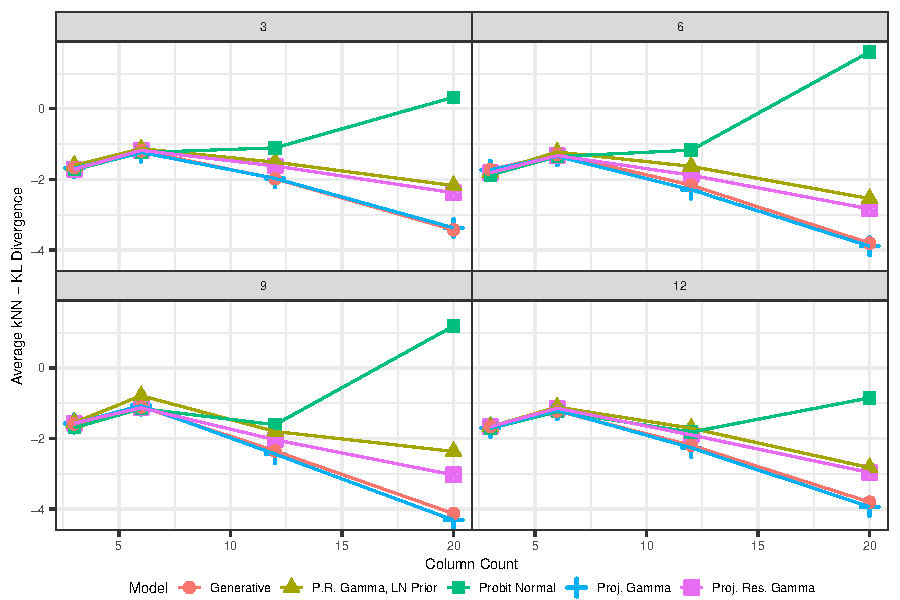
\includegraphics[width=0.9\linewidth]{./images/simulation_knn_kld}
  \end{center}
\end{frame}

\subsection{Integrated Vapor Transport}
\begin{frame}
  \frametitle{IVT - Posterior Predictive Loss}
  \begin{center}
    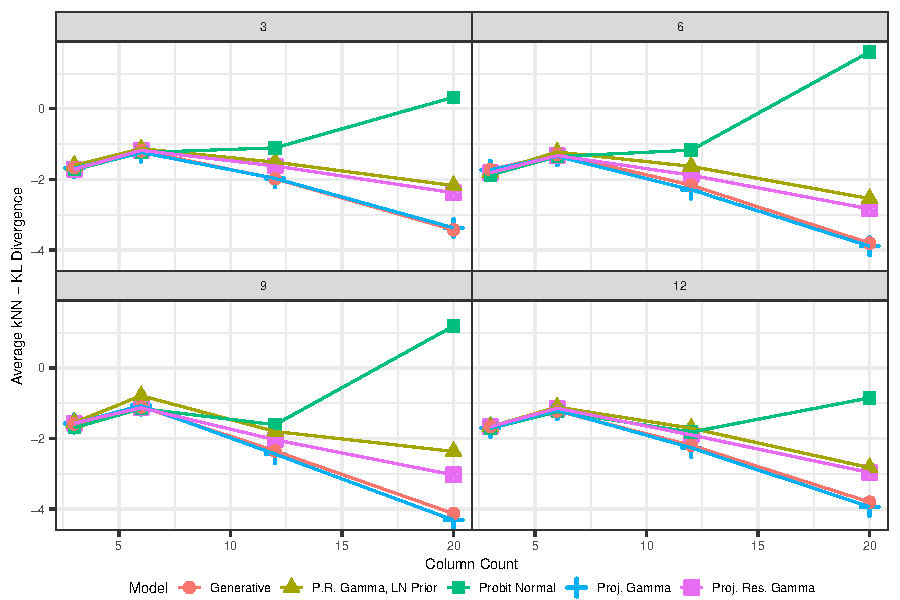
\includegraphics[width=0.9\linewidth]{./images/simulation_knn_kld}
  \end{center}
\end{frame}

\begin{Frame}
  \frametitle{IVT - Energy Score}
  \begin{center}
    
\begin{tabular}{cccccccc}
\toprule
\multicolumn{4}{c}{ } & \multicolumn{2}{c}{dim = 8} & \multicolumn{2}{c}{dim = 46} \\
\cmidrule(l{3pt}r{3pt}){5-6} \cmidrule(l{3pt}r{3pt}){7-8}
Model & Norm & Mix & Prior & PPL & ES & PPL & ES\\
\midrule
Gamma & L1 &  &  & 1.816 & 0.840 & 6.616 & 1.632\\
Gamma & L1 & DP & Gamma & 0.795 & 0.422 & 4.514 & 1.258\\
Gamma & L1 & DP & LogNormal & 0.386 & 0.277 & 2.396 & 0.822\\
Gamma & L1 & M & Gamma & 0.525 & 0.349 & 3.029 & 0.975\\
Gamma & L1 & M & LogNormal & 0.638 & 0.371 & 3.779 & 1.105\\
\addlinespace
Gamma & L2 &  &  & 1.816 & 0.840 & 6.616 & 1.633\\
Gamma & L2 & DP & Gamma & 0.775 & 0.408 & 5.573 & 1.480\\
Gamma & L2 & DP & LogNormal & 0.370 & 0.265 & 2.424 & 0.835\\
Gamma & L2 & M & Gamma & 0.579 & 0.366 & 2.826 & 0.935\\
Gamma & L2 & M & LogNormal & 0.577 & 0.349 & 5.165 & 1.396\\
\addlinespace
Gamma & Linf & DP & Gamma & 0.845 & 0.444 & 6.348 & 1.651\\
Gamma & Linf & DP & LogNormal & 0.384 & 0.278 & 2.376 & 0.823\\
Gamma & Linf & M & Gamma & 0.538 & 0.352 & 3.067 & 0.986\\
Gamma & Linf & M & LogNormal & 0.584 & 0.359 & 3.785 & 1.129\\
Probit Normal &  & DP & Normal & 0.842 & 0.445 & 8.021 & 1.611\\
\addlinespace
Res. Gamma & L1 &  &  & 1.820 & 0.818 & 6.774 & 1.546\\
Res. Gamma & L1 & DP & Gamma & 0.200 & 0.173 & 2.427 & 0.834\\
Res. Gamma & L1 & DP & LogNormal & 0.230 & 0.193 & 1.642 & 0.656\\
Res. Gamma & L1 & M & Gamma & 0.214 & 0.190 & 1.411 & 0.620\\
Res. Gamma & L1 & M & LogNormal & 0.222 & 0.191 & 1.445 & 0.616\\
\addlinespace
Res. Gamma & L2 &  &  & 1.820 & 0.819 & 6.777 & 1.546\\
Res. Gamma & L2 & DP & Gamma & 0.202 & 0.176 & 2.037 & 0.772\\
Res. Gamma & L2 & DP & LogNormal & 0.273 & 0.210 & 1.652 & 0.643\\
Res. Gamma & L2 & M & Gamma & 0.217 & 0.189 & 1.794 & 0.704\\
Res. Gamma & L2 & M & LogNormal & 0.248 & 0.201 & 1.270 & 0.528\\
\addlinespace
Res. Gamma & Linf & DP & Gamma & 0.191 & 0.168 & 2.019 & 0.776\\
Res. Gamma & Linf & DP & LogNormal & 0.228 & 0.191 & 1.458 & 0.589\\
Res. Gamma & Linf & M & Gamma & 0.219 & 0.191 & 1.554 & 0.664\\
Res. Gamma & Linf & M & LogNormal & 0.222 & 0.189 & 1.266 & 0.530\\
\bottomrule
\end{tabular}

  \end{center}
\end{frame}

\begin{frame}
  \frametitle{IVT - KL Divergence}
  \begin{center}
    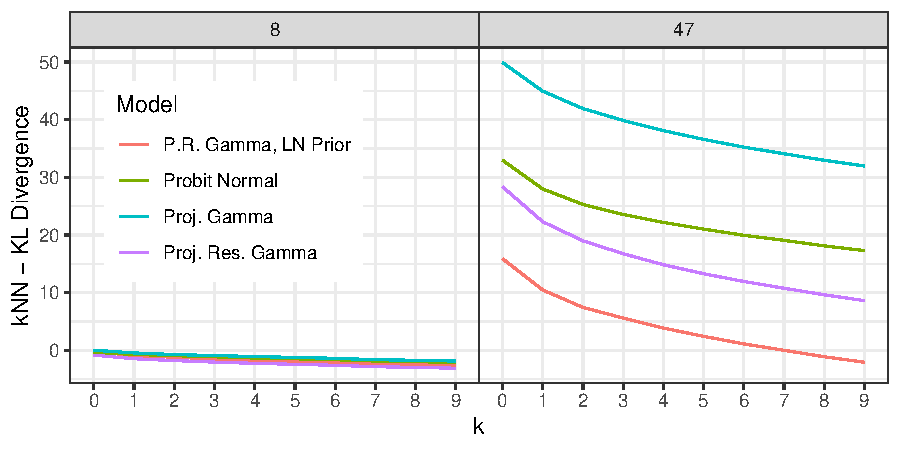
\includegraphics[width=0.9\linewidth]{./images/knn_kld}
  \end{center}
\end{frame}

\section{Applications of EVT Analysis}

\begin{frame}
  \frametitle{Applications of EVT Analysis}
  \begin{itemize}
    \item Pairwise Extremal Dependence Coefficients
    \item Conditional Survival Functions
      \begin{itemize}
        \item Reciprocal of Conditional Return Levels
      \end{itemize}
  \end{itemize}
\end{frame}

\subsection{Pairwise Extremal Dependence Coefficients}

\begin{frame}
  \frametitle{Pairwise Extremal Dependence Coefficients}
    \begin{itemize}
      \item A summary measure of extremal dependence
      \begin{equation*}
        \chi_{kl} = \lim\limits_{u\to\infty}\text{P}\left(Z_k > u\mid Z_l > u\right).
      \end{equation*}
      \pause
      \item Bounded to $[0,1]$
        \begin{itemize}
          \item $0$ represents asymptotic independence
          \item A Pareto model can not represent asymptotic independence
        \end{itemize}
      \pause
      \item Reformulated to unit hypercube
        \begin{equation*}
          \chi_{kl} = \text{E}\left[\frac{V_k}{\text{E}(V_k)}{\bigwedge}\frac{V_l}{\text{E}(V_l)}\right]
        \end{equation*}
    \end{itemize}
\end{frame}

\begin{frame}
  \frametitle{IVT - Extremal Dependence}
  \begin{minipage}{.49\textwidth}
    \centering
    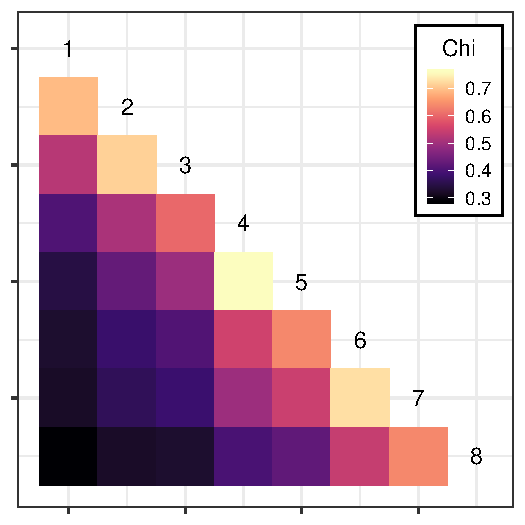
\includegraphics[width=0.99\linewidth]{./images/chi_ij_8}
  \end{minipage}
  \begin{minipage}{.49\textwidth}
    \centering
    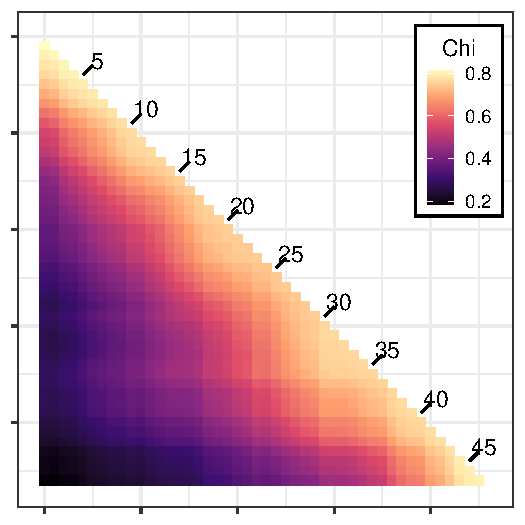
\includegraphics[width=0.99\linewidth]{./images/chi_ij_46}
  \end{minipage}
\end{frame}

\subsection{Conditional survival functions}

\begin{frame}
  \frametitle{Conditional Survival Function}
  \begin{prop}
      In one dimension, the conditional survival curve can be calculated as
   \begin{equation}
      \label{eqn:condsurv1df}
      \text{P}\left[Z_l > z_l\mid {\bf Z}_{\neg(l)} > {\bf z}_{\neg(l)}\right] =
        \frac{\text{E}\left[\wedge_{k = 1}^d \frac{V_k}{z_k}\right]}{
                      \text{E}\left[\bigwedge_{k \neq l}\frac{V_k}{z_k}\right]}
    \end{equation}
      where $\bm{V} = \bm{Z} / \pnorm{\bm{Z}}{\infty}$.
  \end{prop}
\end{frame}

\begin{frame}
  \frametitle{Conditional Survival Function - Cont.}
  \begin{equation}
    \label{eqn:condsurv1d}
    \text{P}\left[Z_l > z_l\mid {\bf Z}_{-(l)} > {\bf z}_{-(l)}\right] =
      \frac{\text{P}\left[\cap_{k = 1}^d Z_k > z_k\right]}{\text{P}\left[\cap_{k \neq l} Z_k > z_k\right]}.
  \end{equation}
  \pause
  $R = \pnorm{{\bf Z}}{\infty}$, ${\bf V} = \frac{{\bf Z}}{R}$, such that
    ${\bf V}\in \mathcal{S}_{\infty}^{d-1}$.  Then ${\bf Z} = R{\bf V}$.
  \begin{equation}
    \text{P}\left(\cap_{k = 1}^d Z_k > z_k\right) = \text{P}\left(\cap_{k = 1}^d RV_k > z_k\right)
  \end{equation}
  \pause
  Recall, for standard Pareto, $\text{P}(R > r) = 1\wedge\frac{1}{r}$.
  \begin{equation}
    \text{P}\left[\bigcap_{k = 1}^d R > \frac{z_k}{v_k}\right] =
      \text{P}\left[R  > \bigvee_{k=1}^d\frac{z_k}{V_k}\right] =
      \text{E}\left[1 \bigwedge \left(\bigvee_{k = 1}^d\frac{z_k}{V_k}\right)^{-1}\right]
  \end{equation*}
  $V_k \in [0,1]$; $z_k > 1$ (for the region of interest) $\implies$ $\frac{z_k}{V_k} > 1$
  \pause
  \begin{equation}
    \text{P}\left[\cap_{k = 1}^d Z_k > z_k\right] = \text{E}\left[\wedge_{k = 1}^d\frac{V_i}{z_i}\right].
  \end{equation}
  \pause
  And similar for the denominator
  \begin{equation}
    \text{P}\left[Z_l > z_l\mid {\bf Z}_{\neg(l)} > {\bf z}_{\neg(l)}\right] =
      \frac{\text{E}\left[\wedge_{k = 1}^d \frac{V_k}{z_k}\right]}{\text{E}\left[
                \bigwedge_{k \neq l}\frac{V_k}{z_k}\right]}
  \end{equation}
\end{frame}

\begin{frame}
  \frametitle{IVT - Conditional Survival 1d}
  \begin{center}
    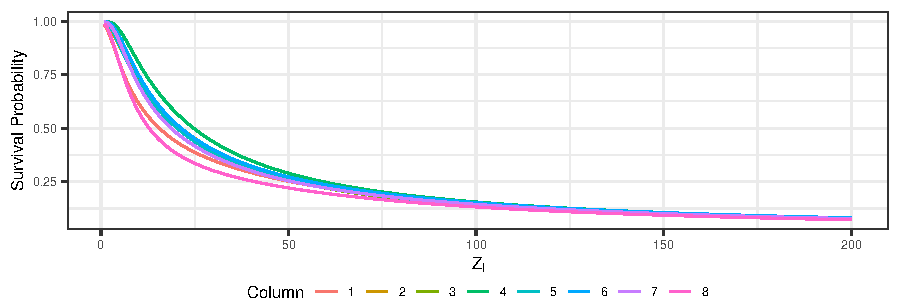
\includegraphics[width = 5in]{./images/condsurv_1d}
  \end{center}
\end{frame}

\begin{frame}
  \frametitle{IVT - Conditional Survival 2d (selected)}
  \begin{center}
    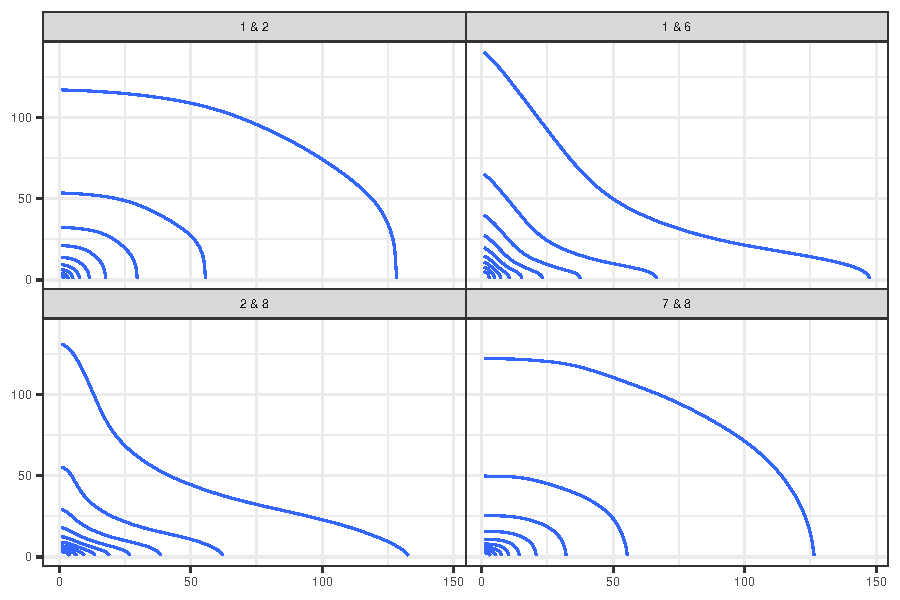
\includegraphics[width = 5in]{./images/condsurv_2d}
  \end{center}
\end{frame}

\section{Applications to anomaly detection}

\begin{frame}
  \frametitle{What is an anomaly?}
  \begin{itemize}
    \items Anomalies are:
      \begin{itemize}
        \item Observations with large outliers?
        \item Observations with outsized effects?
        \item Data that is \emph{different}.
        \item Data from regions of data sparsity
      \end{itemize}
    \item Desire anomaly \emph{scores}--larger$\righarrow$more anomalous
  \end{itemize}
\end{frame}

\begin{frame}
  \frametitle{Classical Anomaly Detection Methods}
  \begin{itemize}
    \item Clustering methods
      \begin{itemize}
        \item Linkage-based (single, \dots, complete)
        \item Centroid-based ($k$-Means)
        \item Density-based (DBSCAN)
      \end{itemize}
    \item Non-statistical Models
      \begin{itemize}
        \item Isolation Forest
        \item One-class SVM
        \item Local Outlier Factor
      \end{itemize}
    \item Statistical Models
      \begin{itemize}
        \item Gaussian mixture models
        \item If you can generate a density directly\dots
      \end{itemize}
  \end{itemize}
\end{frame}

\begin{frame}
  \frametitle{Proposed Anomaly Scoring Methods}
  \begin{itemize}
    \item Density Estimation on the hypersphere
    \item Contribution to Posterior Predictive Loss
  \end{itemize}
\end{frame}

\begin{frame}
  \frametitle{Density Estimation on the Hypersphere}
  \begin{itemize}
    \item Sample from posterior predictive distribution
    \item Density based on \emph{distance} to $k$th nearest neighbor
    \begin{equation}
        S_{i,(k)}^{-1} =
          \frac{k}{N}\frac{\Gamma\left(\frac{d-1}{2} - 1\right)}{\pi^{\frac{d-1}{2}}D_{k}^{d-1}(V_i)}
    \end{equation}
  \end{itemize}
\end{frame}

\begin{frame}
  \frametitle{Anomaly Detection Results (Simulated Data)}
  \begin{center}
    
\begin{tabular}{ccccccc}
\toprule
\multicolumn{2}{c}{ } & \multicolumn{2}{c}{Proposed} & \multicolumn{3}{c}{Classic} \\
\cmidrule(l{3pt}r{3pt}){3-4} \cmidrule(l{3pt}r{3pt}){5-7}
nMix & nCol & kNN & PPL & o.c.SVM & L.O.F. & I.Forest\\
\midrule
5 & 5 & 0.750 & 0.734 & 0.511 & 0.596 & 0.508\\
5 & 10 & 0.754 & 0.711 & 0.554 & 0.740 & 0.524\\
10 & 5 & 0.532 & 0.543 & 0.574 & 0.599 & 0.563\\
10 & 10 & 0.605 & 0.593 & 0.509 & 0.544 & 0.459\\
\bottomrule
\end{tabular}
  \end{center}
\end{frame}

\section{Scaling to higher dimensions}

\begin{frame}
  \frametitle{Scaling to Higher Dimensions}
  \begin{itemize}
    \item Compuitational advances in modelling
      \begin{itemize}
        \item Variational Bayes
      \end{itemize}
    \item Maintaining Model Fidelity at Scale
      \begin{itemize}
        \item Gaussian Mixture on $\log\alpha$
        \item $\eta$-Cones
      \end{itemize}
  \end{itemize}
\end{frame}

\begin{frame}
  \frametitle{Scale - Mixture of Gammas Prior}
  \begin{itemize}
    \item $\eta \subset \lbrace 1,\ldots,d\rbrace$.  Define the $\eta$-Cone:
      \begin{equation*}
        \mathcal{C}_{\eta} = \left\lbrace \bm{z} : z_l > 0 \text{ for }l\in\eta;
                              \hspace{0.2cm} z_l = 0 \text{ for }l\not\in\eta\right\rbrace
      \end{equation*}
    \pause
    \item Gamma models do not have support at 0--$\epsilon$-thickened cones
      \begin{equation*}
        \mathcal{C}_{\eta}^{(\epsilon)} = \left\lbrace \bm{z} : z_l \geq \epsilon
          \text{ for }l\in\eta; \hspace{0.2cm} z_l = 0 \text{ for }l\not\in\eta\right\rbrace
      \end{equation*}
    \pause
    \item How does this help us?
      \begin{itemize}
        \item For Gamma models, $\alpha < 1$ $\implies$ mass near 0
        \item A mixture of gammas for $\alpha_l$:
          \begin{equation*}
            \alpha_l \sim I_{l\in\eta}\text{Ga}(\alpha_l\mid a_1, 1)
                        + I_{l\not\in\eta}\text{Ga}(\alpha_l\mid a_0, 1)
          \end{equation*}
          with $\alpha_0 < 1$, $\alpha_1 > 1$
      \end{itemize}
  \end{itemize}
\end{frame}

\section{Conclusion}

\begin{frame}
  \frametitle{Conclusion}
  \begin{itemize}
    \item Developed a means of describing the dependence structure of the multivariate Pareto
    \item Demonstrated inherent difficulty in distribution on $\mathcal{S}_{\infty}^{d-1}$
      \begin{itemize}
        \item developed a means of model comparison on the space
      \end{itemize}
    \item Applied models to IVT data
      \begin{itemize}
        \item Pairwise Extremal Dependence Coefficients
        \item Conditional Survival Curves
      \end{itemize}
    \item Anomaly Detection (Preliminary)
    \item Modelling at Scale (on the horizon)
  \end{itemize}
\end{frame}

\end{document}
